\documentclass[../SustainableHEP.tex]{subfiles}
\graphicspath{{\subfix{Sections/Figs/}}}
\begin{document}
\RaggedRight
\sloppy
%%%%%%%%%%%%%%%%%%%%%%%%%%%%%%%%%%%%%%%%%%%%%%%%%%

\newpage
\section{Energy}
\label{sec:Energy}

\exSum

%%%%%%%%%%%%%%%%%%%%%%%%%%%%%%%%%%%%%%%%%%%%%%%%%%

\begin{figure}
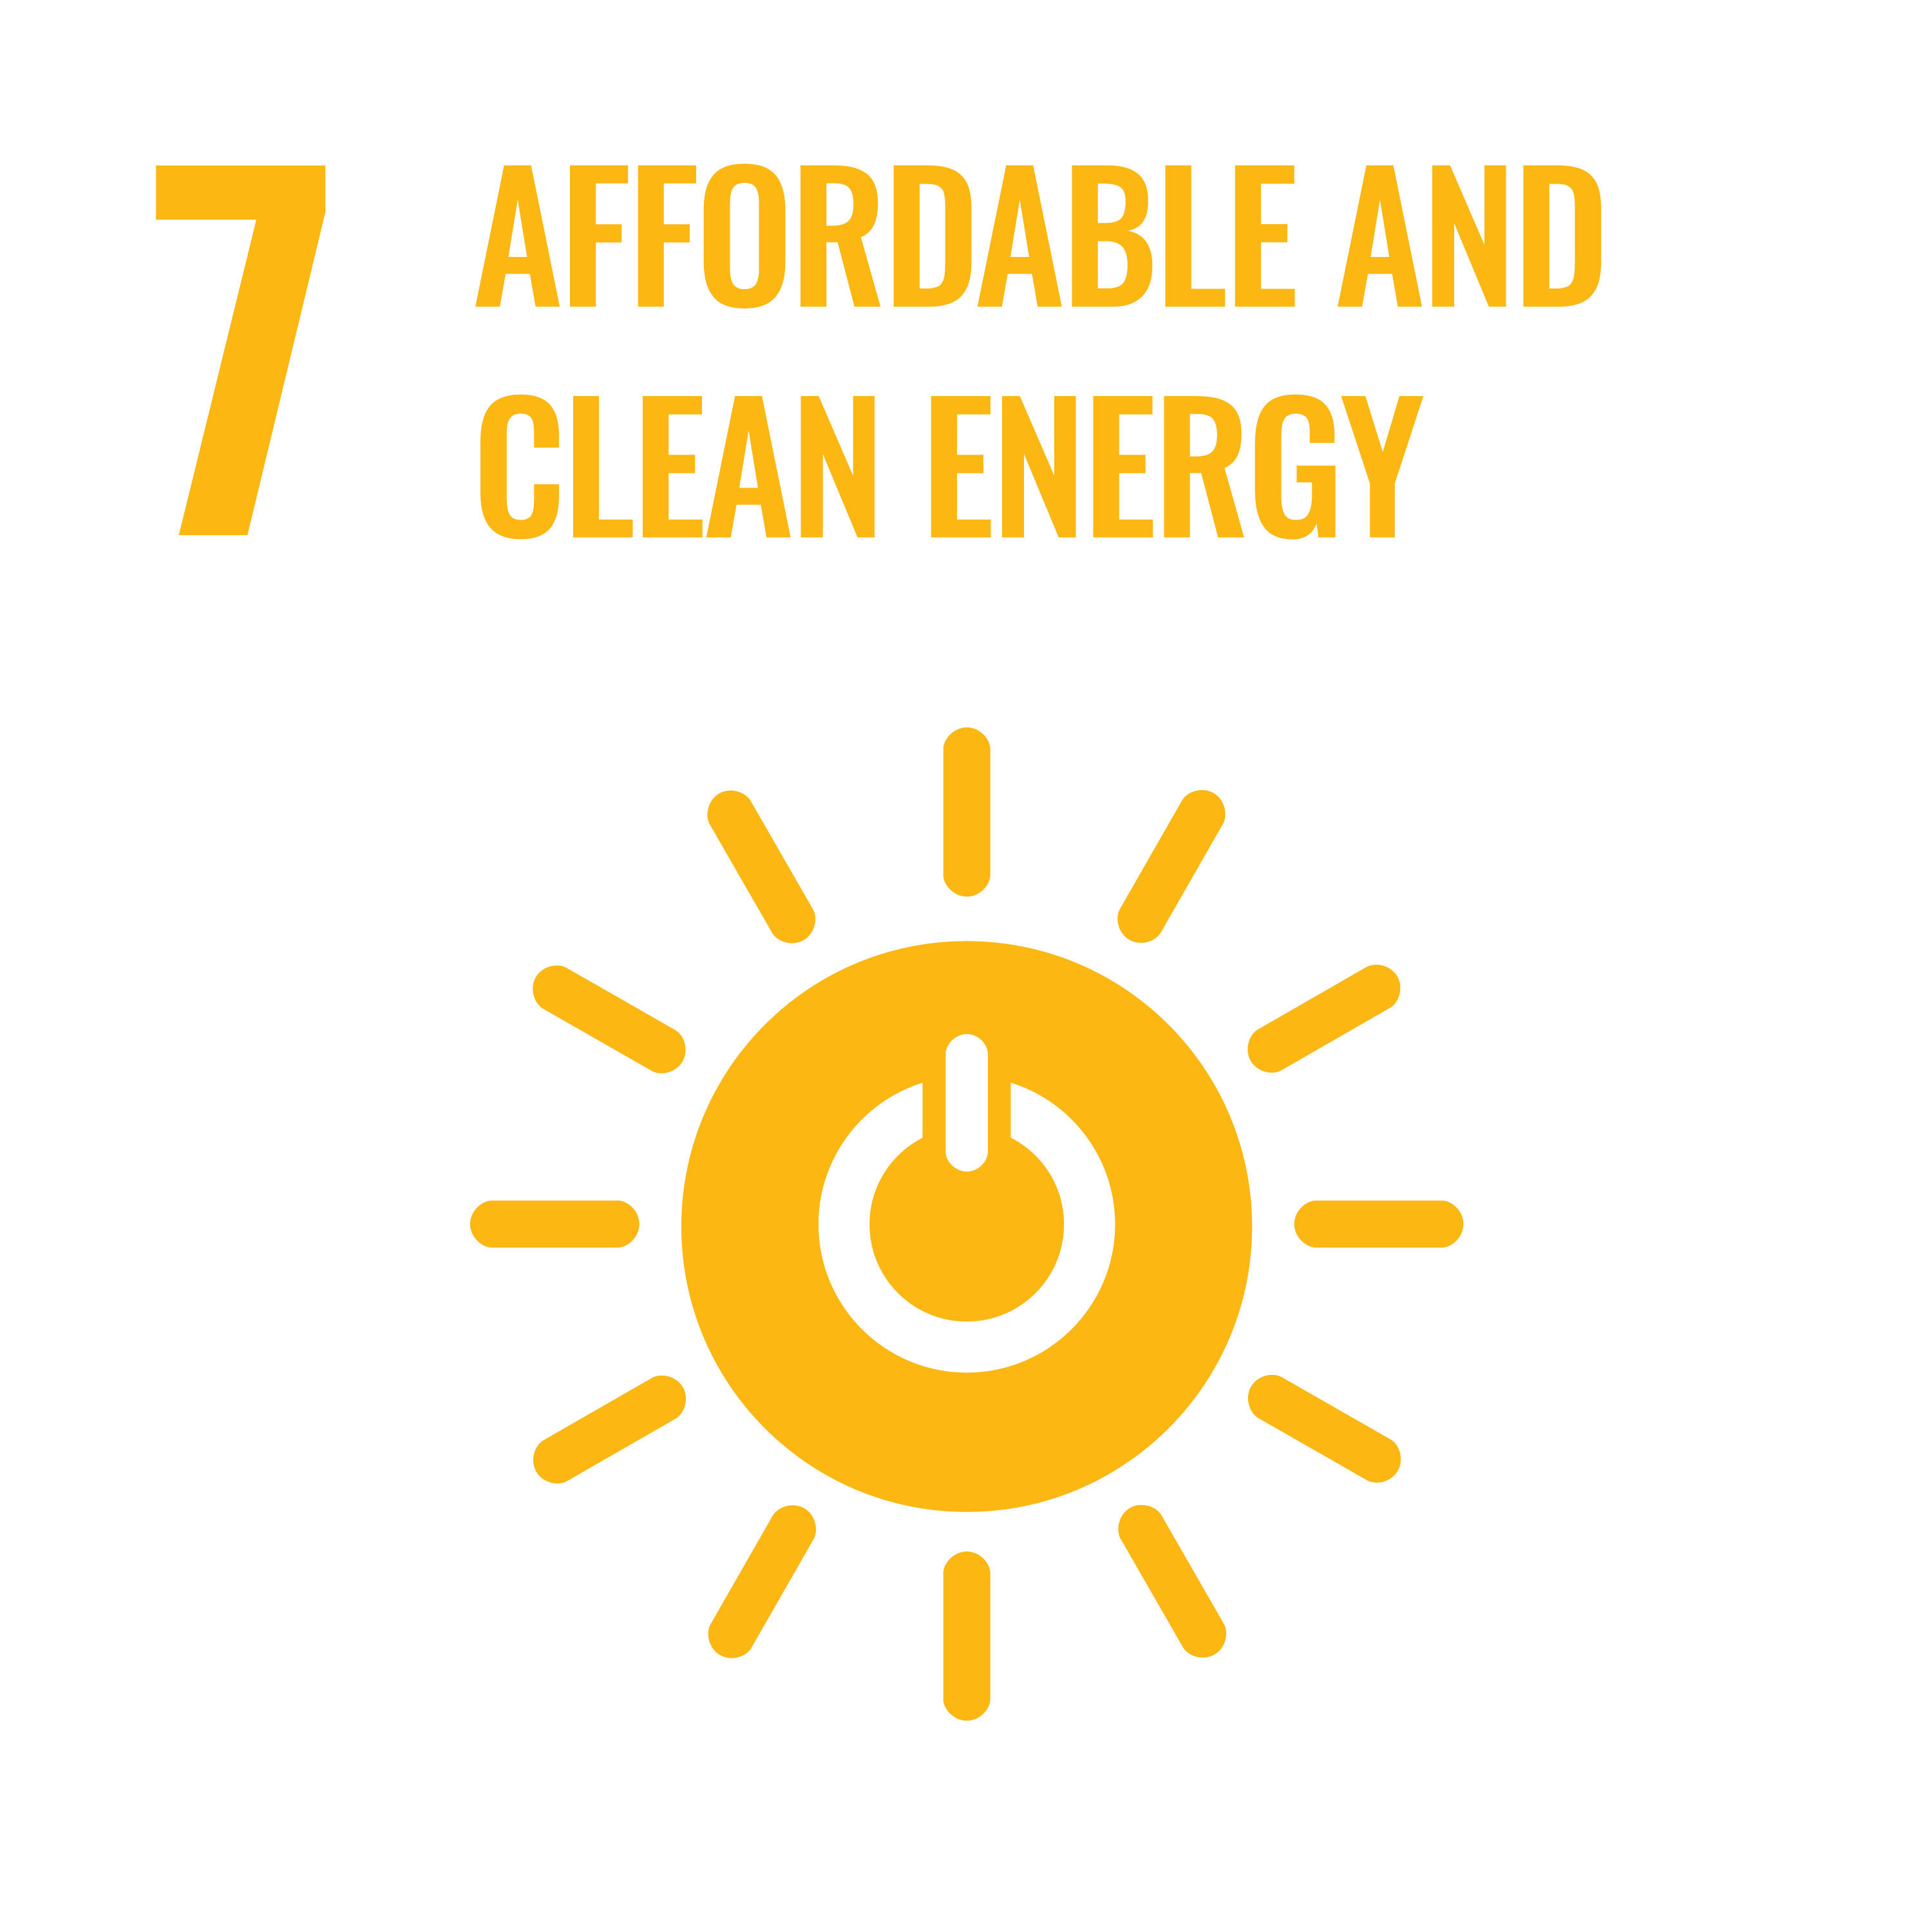
\includegraphics[width=\SDGsize]{Sections/Figs/Common/SDG_7_CleanEnergy.png}~%

\includegraphics[width=\SDGsize]{Sections/Figs/Common/SDG_9_IndustryInnovation.png}~%

\includegraphics[width=\SDGsize]{Sections/Figs/Common/SDG_11_SustainableCities.png}~%
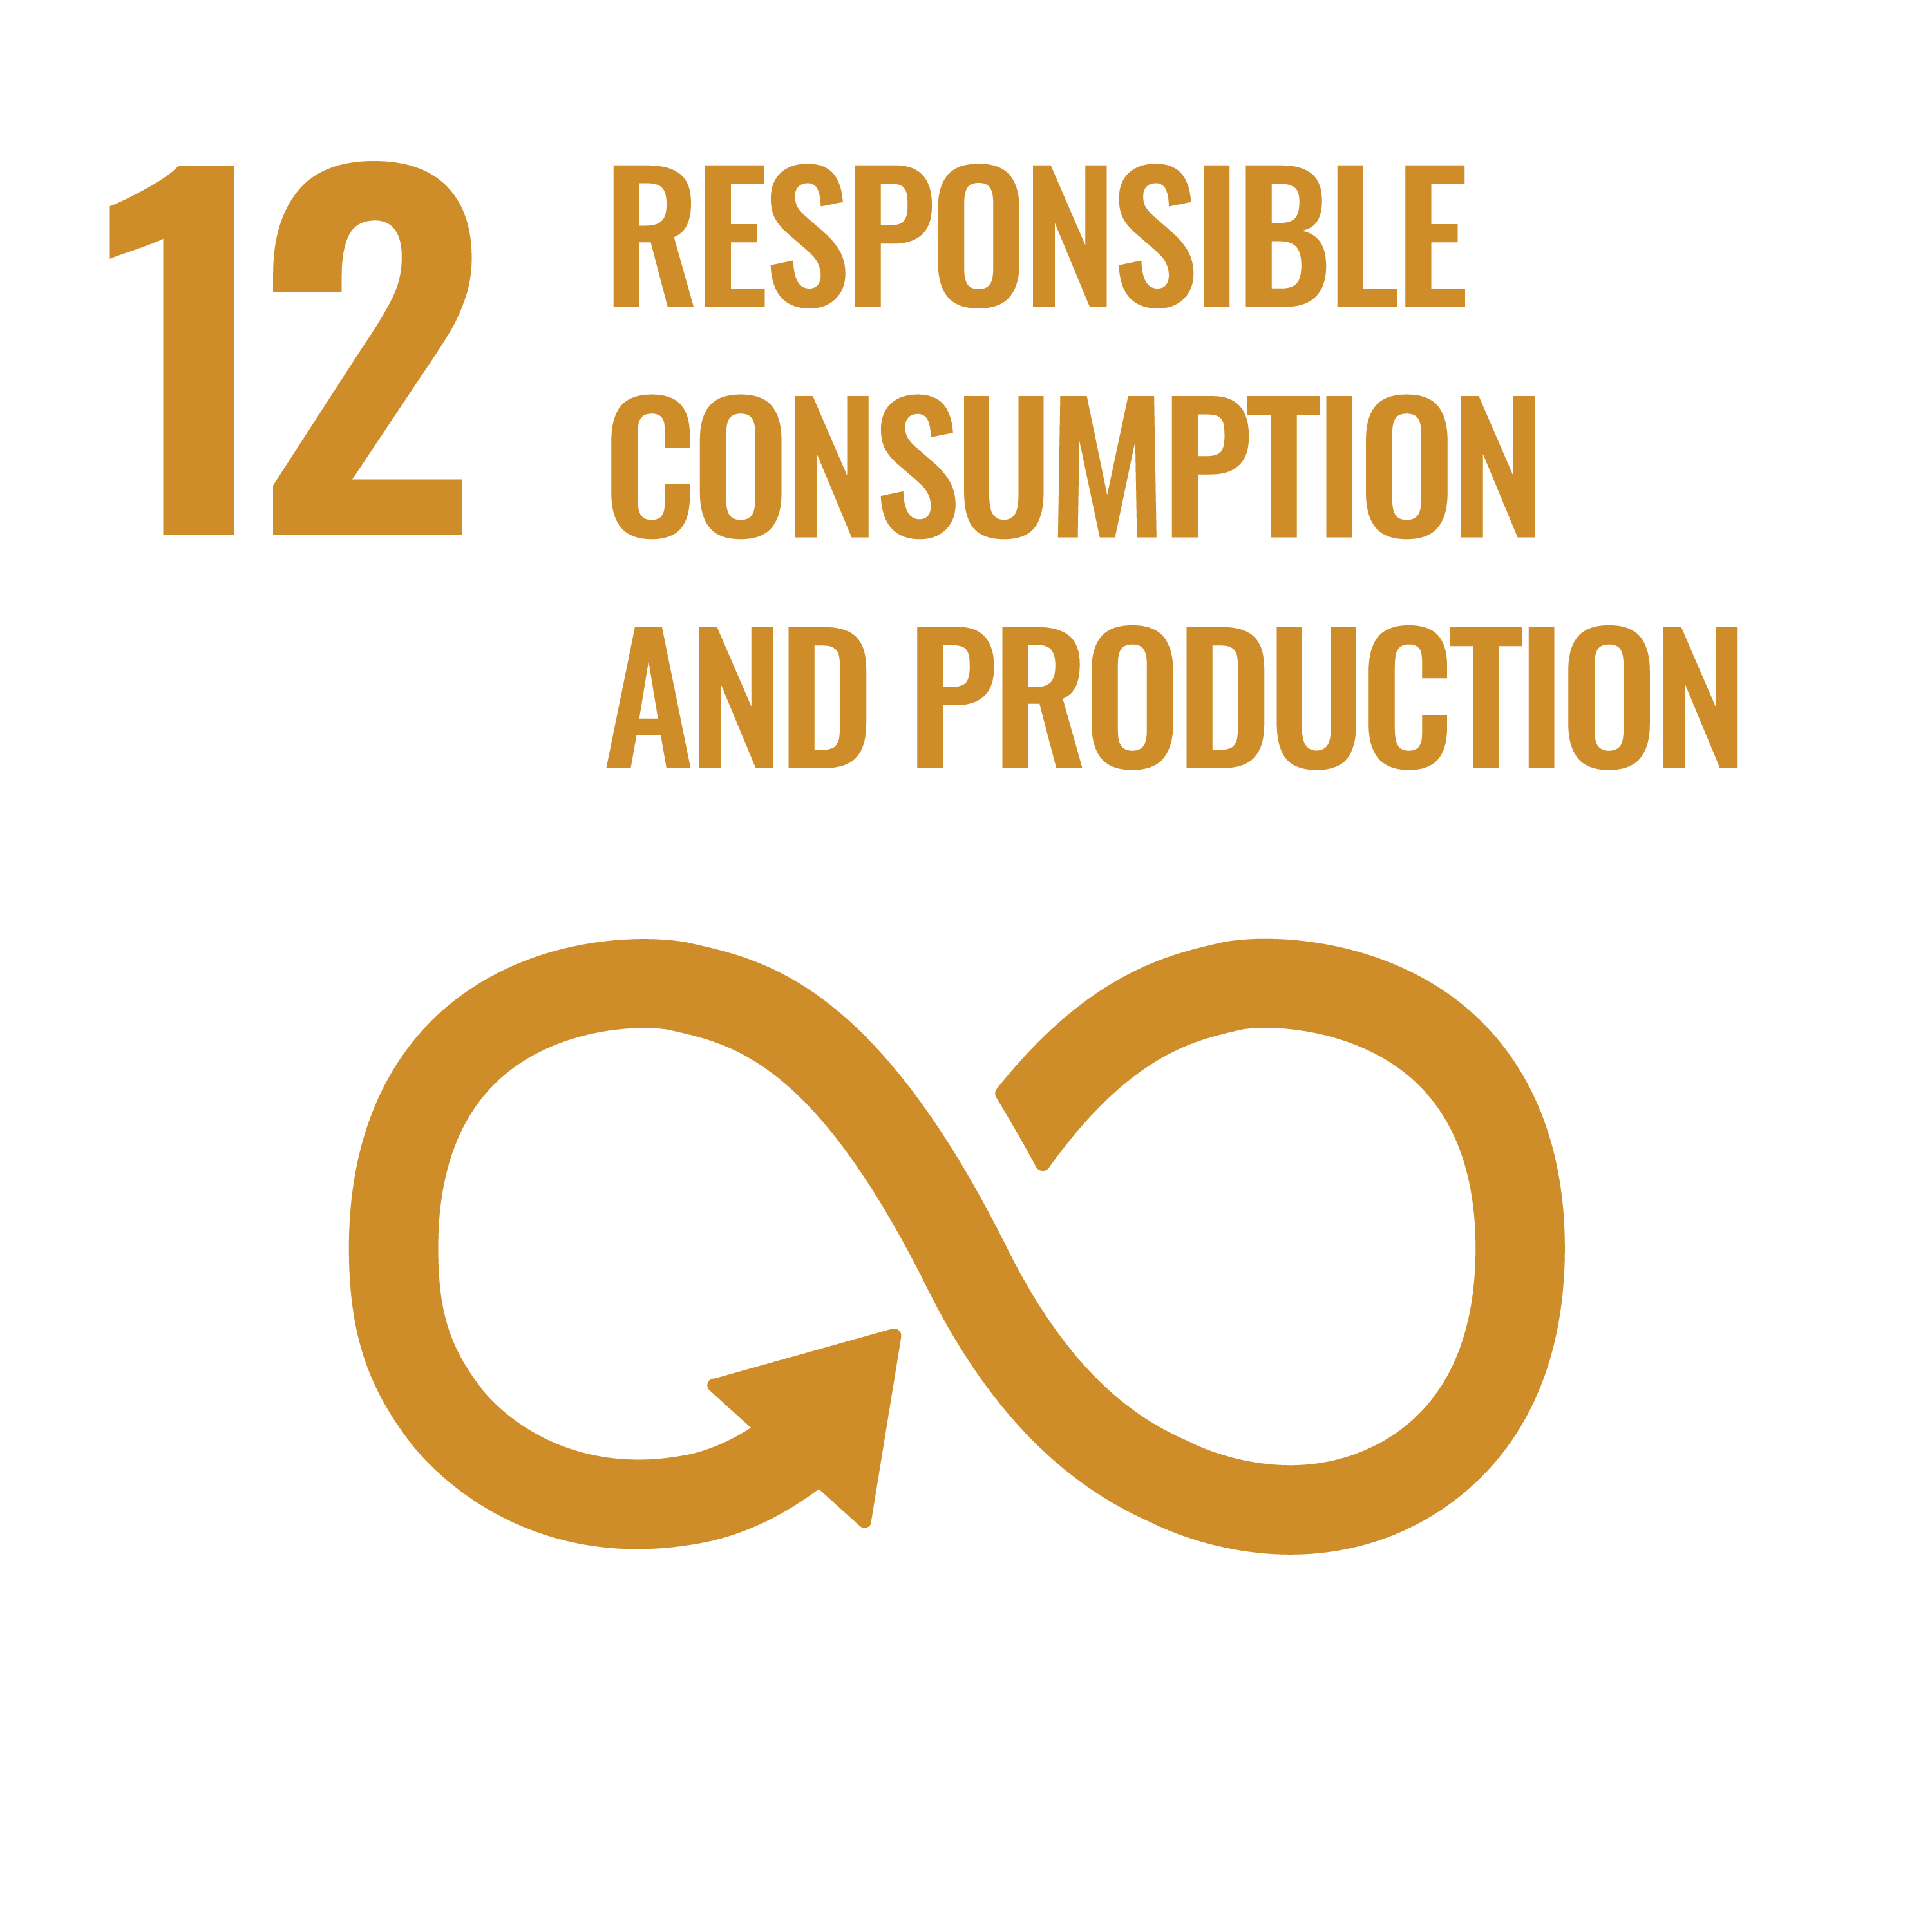
\includegraphics[width=\SDGsize]{Sections/Figs/Common/SDG_12_ResponsibleConsumption.png}~%

\includegraphics[width=\SDGsize]{Sections/Figs/Common/SDG_13_ClimateAction.png}~%

\includegraphics[width=\SDGsize]{Sections/Figs/Common/SDG_16_PeaceJusticeStrongInstitutions.png}~%

\includegraphics[width=\SDGsize]{Sections/Figs/Common/SDG_17_PartnershipForGoals.png}

\end{figure}

%%%%%%%%%%%%%%%%%%%%%%%%%%%%%%%%%%%%%%%%%%%%%%%%%%

\noindent
The operation of experimental equipment and computing facilities at large-scale research centres has a significant energy footprint. 
In addition, energy is required for the construction and disassembly of infrastructure, for heating and cooling buildings, and for transport of goods and people. To comply with the Paris Agreement, future facilities must be effectively climate-neutral, and this presents a significant challenge for \acrshort{hecap}.

Particle collider experiments are particularly power-hungry, with the \acrshort{lhc} at \acrshort{cern} being a prominent example. With its particle accelerators, detectors and extensive infrastructure, CERN consumes up to 1,300~GWh of electricity annually, of which 55\% is due to LHC operations~\cite{Environment:2737239,CERNenergymanagement}. CERN plans to significantly increase the scale of its installations in a push towards higher energies and intensities. Doing so responsibly will require a concerted effort to minimise power consumption and increase the energy efficiency of the infrastructure, and a careful analysis of how to source the remaining energy needs sustainably.

CERN receives most of its electricity from the French grid, which is currently characterised by a high share of low-carbon nuclear power, suppressing its electricity-related \CdO\ emissions in comparison with other facilities  (see \fref{fig:Intro-ComparativeEmissions}).\footnote{CERN's annual electricity emissions range from 9,000 \acrshort{tco2e} (LHC in shutdown) to 15,000 \tCdOe\ (LHC in operation)~\cite{Environment:2737239}.} However, taking into consideration the decreasing share of nuclear power in the French grid over the last 15 years, as well as the wider common European electricity market, where fossil fuels account for 37\% of electricity production on average~\cite{BPReport}, the outlook is more worrying.\footnote{For a live visualisation of the carbon emissions of electricity by country, see Ref.~\cite{ElectricityMap}.}

It is important to place the energy needs of \ACR\ research infrastructure within the context of the world's necessary and rapid transition to zero-carbon energy sources. Global primary energy consumption in 2019 was approximately 160,000~TWh (equivalent to an average power consumption of 18,000~GW), around 80\% of which comes from \CdO-emitting fossil fuels~\cite{OWDfuels}. Moreover, demand is rising, primarily due to the growth and industrialisation of emerging countries.  A 50\% reduction of \CdO\ emissions by 2030, as stipulated in the Paris Agreement in combination with the latest \acrshort{ipcc} scenarios (see~\fref{fig:ene-netco2}), will create a huge global energy gap, as shown in \fref{fig:ene-gap}~\cite{physikkonkret}. 

%%%%%

\begin{figure}[!ht]
     \centering
    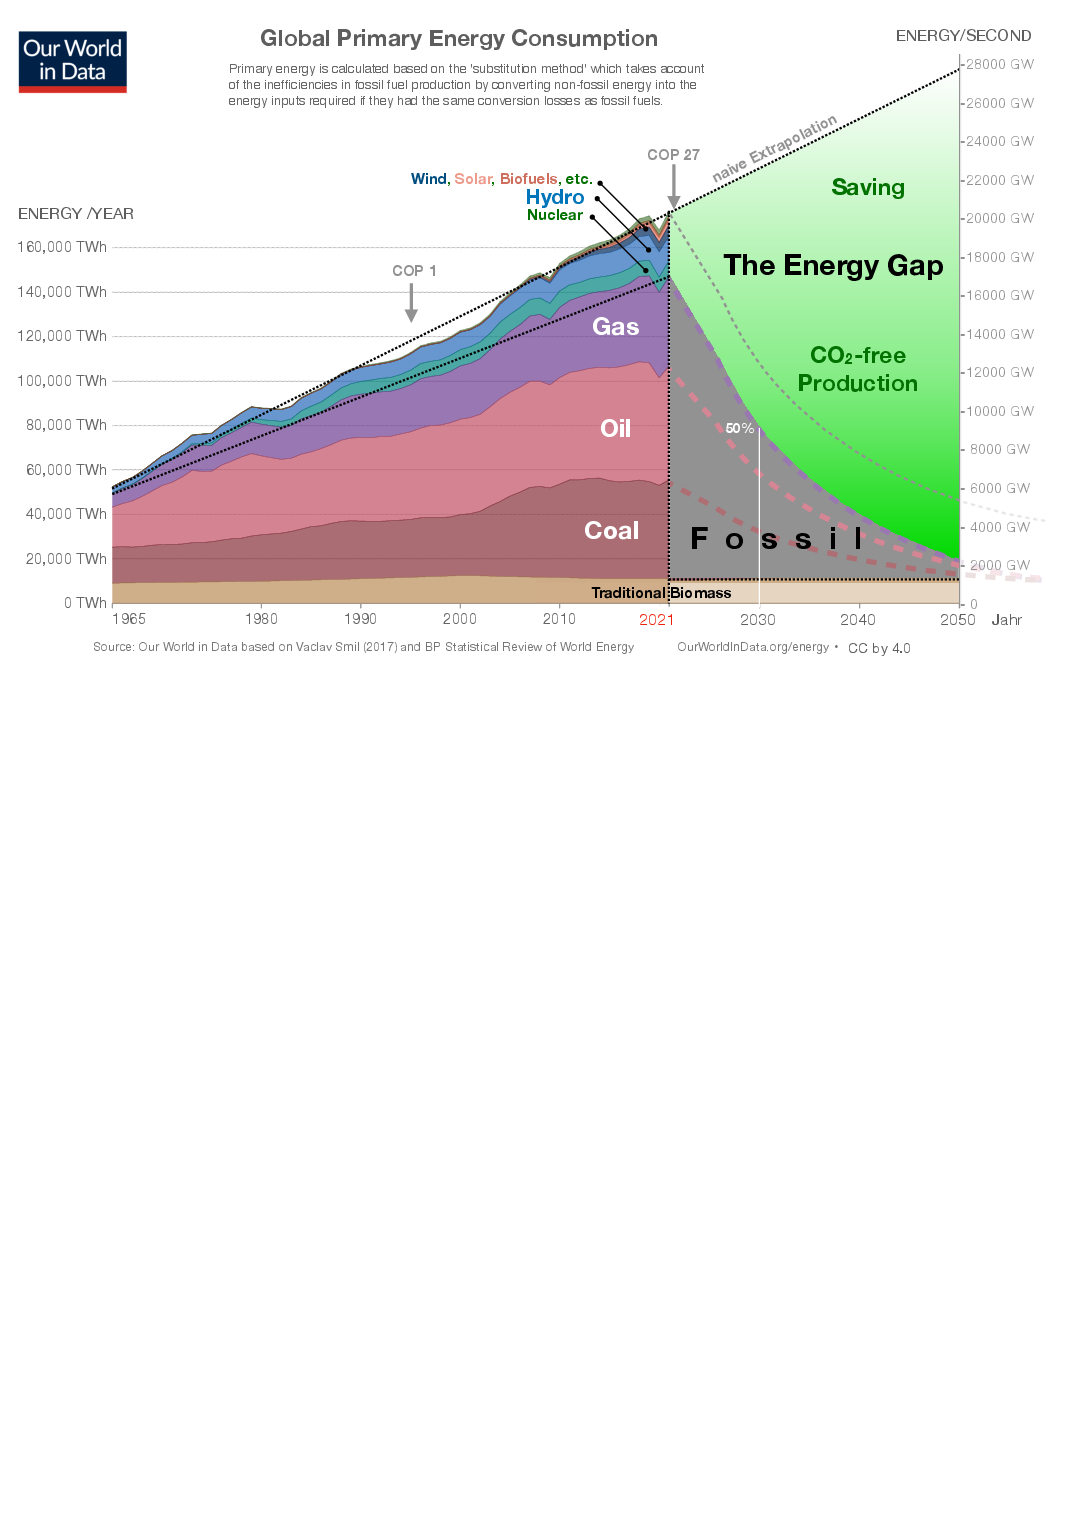
\includegraphics[width=0.9\linewidth]{Energy/ene-gap.png}     
    \caption[Primary energy consumption is dominated by fossil fuels]%
        {Global primary energy consumption is dominated by fossil fuels, the use of which has been increasing steadily despite repeated warnings from the climate change conferences of the United Nations (COP) dating as far back as 1995. Decreasing emissions by 50\%, as recommended by the IPCC to avoid irreversible tipping points~\cite{OECDTippingPoints} (see blue line in \fref{fig:ene-netco2}) creates a large energy gap that must be filled by additional climate-neutral power generation, or by energy savings and recuperation. Consumption was extrapolated linearly from 1965--2021 to account for additional demand from emerging countries. Left part of figure taken from Ref.~\cite{OWDgap}, based on data from Refs.~\cite{Smil,BP2022}, reused and adapted under the terms of the \href{https://creativecommons.org/licenses/by/4.0/}{Creative Commons Attribution 4.0 International (CC BY 4.0) license}.\label{fig:ene-gap}}
 \end{figure}

%%%%%

Many experimental technologies such as \CdO\ capture and storage (CCS) will not be viable for large-scale implementation within this short time frame~\cite{IPCCMitigationReport}. Filling the energy gap with solar, wind, and nuclear power requires upscaling existing facilities by more than an order of magnitude within seven years, a not inconsiderable task. Therefore, substantial energy savings and efficiency increase will be indispensable. Even tripling the output of existing solar, wind and nuclear installations by 2030 (which may itself be unrealistic), the fossil energy gap would still require a 40\% global efficiency increase compared to today. Substantial savings in energy require systemic changes in technology and behaviour, such as transitioning from combustion engines to electric motors, from gas heating to heat pumps and from cars to rail. The global situation is therefore likely to result in energy becoming scarce and expensive in the coming decades, with the potential to directly limit our capabilities to conduct energy-intensive experiments and data analysis in basic research.

This chapter focuses on potential sources of sustainable energy for \ACR\ research infrastructure in \sref{sec:Ene-Transition}, and energy savings and recuperation in \sref{sec:Ene-Saving}. Saving energy through structural and organisational changes are described elsewhere: see \sref{sec:Computing} for computing, \sref{sec:Travel} for mobility, and \sref{sec:Waste} for procurement.

%%%%%%%%%%%%%%%%%%%%%%%%%%%%%%%%%%%%%%%%%%%%%%%%%%

\clearpage

\begin{reco2}{\currentname}
{
\begin{itemize}[leftmargin=6 mm]
\setlength{\itemsep}{\recskip}
\item Save energy in all ways practicable, e.g., by avoiding unnecessary heating or cooling of workspace, and by turning off electrical items when not in use.

\item Read the sections about computing (\sref{sec:Computing}) and mobility (\sref{sec:Travel}).

\end{itemize}
}
{
\begin{itemize}[leftmargin=6 mm]
\setlength{\itemsep}{\recskip}
\item Ensure that energy efficiency is a major focus in experimental design, and prioritise technologies that minimise consumption and maximise energy recovery.

\item Monitor, report, and assess energy usage with the aim of reducing consumption and resulting emissions.

\item Read the section on research infrastructure and technology (\sref{sec:Technology}).
\end{itemize}
}
{
\begin{itemize}[leftmargin=6 mm]
\setlength{\itemsep}{\recskip}
\item Ensure that energy efficiency is a major factor in the renovation of existing estates and the design and construction of new infrastructure.

\item Prioritise moving to renewable energy sources via both local generation, and energy import and export.

\item Collate and publish energy usage and emissions statistics, stratifying by source, e.g., heating, experimental infrastructure, computing, transportation, and procurement.

\item Lobby for environmentally sustainable energy policy.
\end{itemize}}

\end{reco2}

%%%%%%%%%%%%%%%%%%%%%%%%%%%%%%%%%%%%%%%%%%%%%%%%%%

\newpage

\subsection{Low-Carbon Energy}
\label{sec:Ene-Transition}

Transitioning the energy demands of \ACR\ research to \CdO-neutral sources will likely require a mix of sources: solar, wind, hydro, geothermal, and nuclear power, many of which will be strongly location-dependent. Despite their relatively low cost (see \fref{fig:ene-mitigation}), the
geographical and geological limitations of renewable energy, combined with the challenge that significantly increasing the share of nuclear power presents (see \csref{cs:nuclear_gap} for details), make a rapid transition to carbon-neutral energy impossible for \ACR\ without some large-scale transmission or import of sustainable energy. Alternatively, efforts could be made to site future facilities near abundant sources of renewable energy, which could have the additional benefit of contributing to the local economy over a longer period. The Synchrotron-Light for
Experimental Science and Applications in the Middle East (\acrshort{sesame}) project ~\cite{Sesame} is one example.  World-leading research centres like \acrshort{cern},  with their history of cooperation across political and ideological boundaries, are uniquely placed to spearhead such initiatives.  

\begin{figure}[!tb]
     \centering
     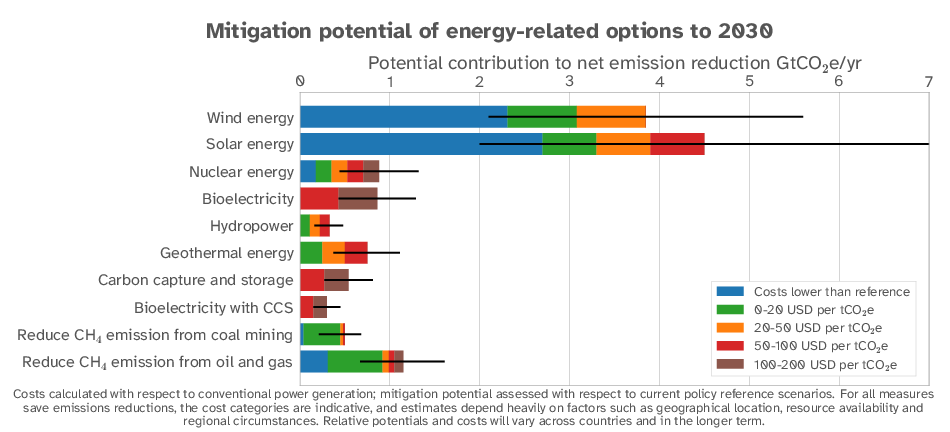
\includegraphics[width=0.99\linewidth]{Sections/Figs/Energy/IPCCMitigationPotential.png}
     \caption[IPCC 
    mitigation potential for alternative sources of energy]{Overview of energy-related mitigation options and their estimated range of costs and potentials in 2030, as determined by the IPCC in their Sixth Assessment Report. All costs were calculated with respect to conventional power generation; potentials were assessed with respect to the reference scenario in the World Energy Outlook 2019~\cite{IEA2019}.  Data source: IPCC WGIII Summary for Policy Makers, Figure SPM.7, Ref.~\cite{IPCCMitigationData}.  For further details on how the data was obtained, see Supplementary Material 12.SM.1.2 in Ref.~\cite{IPCCMitigationReport}.}
     \label{fig:ene-mitigation}
 \end{figure}

\paragraph{Solar}

Solar energy is abundant, and near-universally available.  Its intensity depends on latitude, with the highest efficiencies in the deserts of the sun belts north and south of the equator. According to a 2021 report by the Carbon Tracker Initiative~\cite{CarbonTracker21}, populating an area of only 450,000 km$^2$ with solar panels would be sufficient to satisfy global energy demands.  This corresponds to an area the size of Morocco, two-thirds that of Texas, or 4\% of European landmass.\footnote{Surprisingly, the report also states that there is at most a factor of two difference between the hours of full sunlight available in most countries on our planet (Namibia and Ireland representing two extremes, excluding Iceland).}  According to the IPCC~\cite{IPCCMitigationReport}, ``The global technical potential of direct solar energy far exceeds that of any other renewable energy resource and is well beyond the total amount of energy needed to support ambitious mitigation over the current century.''  Large-scale adoption of photovoltaic (PV) panels poses concerns due to resource use, particularly the energy-intensive production of silicon used to produce the panels, and end-of-life waste generation.  These impacts can be partially mitigated by material recovery in PV cell recycling, and their reuse~\cite{DANIELAABIGAIL2022103539}.

Solar panels are also easily retrofitted onto existing infrastructure, and their price has dropped by almost 90\% in the last two decades.  Unfortunately, solar power can be unavailable when it is needed most:\ at night and during winter (in countries at higher latitudes), leading to a need to increase its efficiency and storage capacity (see \sref{subsec:grid}). See \csref{case:solar} for a study of the implementation of in-house solar power at CERN.

\paragraph{Wind}

By comparison with solar energy, wind energy is more sensitive to local conditions. In Europe, competitive locations for wind energy, with costs below \EUR{0.06} per kWh, are primarily offshore, and are concentrated along the coasts of the North and Baltic Seas, the Bay of Biscay, and the English Channel~\cite{EEAWindEnergy}.
Landlocked countries, such as Switzerland or Austria, are generally less suited for production of energy through wind turbines. Producing 25\% of, \eg Swiss energy demand from wind power would require populating 100\% of its agricultural farmland with wind turbines (although this does not preclude growing crops beneath the windmills).  By contrast, fulfilling a quarter of Danish or Estonian energy demand would require less than 4\% of the farmland~\cite{EEAWindEnergy}. 

\paragraph{Hydroelectric}

Water power is even more reliant on local conditions, such as high flows or water volumes and large altitude difference, which naturally limits its applicability.  However, the energy output of hydroelectric plants is steady, and can be adjusted to demand very quickly, making it a good complement to other renewable sources. It can also be used for energy storage, see \sref{subsec:grid}. The largest hydroelectric capacity is in China, which produces almost 30\% of the global hydroelectric power~\cite{IHA2021}, thanks to its large projects in the Yangtze River valleys.

Mega-dams, however, constitute a large intervention on the natural environment, and consequently come with associated risks, such as landslides, earthquakes, and destruction of habitats, and can themselves be a source of the potent \acrshort{ghg} methane when flooded flora rots. The Three Gorges dam in particular has been controversial both domestically and abroad~\cite{ThreeGorges}. In arid areas, or during periods of drought, which are expected to become more prevalent due to climate change, hydroelectric power may be in competition with agricultural needs, and climate change may jeopardise future yields of existing dams.

While the potential for marine power generation from ocean currents, tides, waves, and gradients in salt and temperature (collectively known as Ocean Energy Technologies) is huge, there is no technology currently mature enough to produce marine power at large scale~\cite{OET}.

\paragraph{Geothermal}

Geothermal energy is a stable source of renewable energy. It consists of residual heat from the time when the Earth was formed and of heat newly produced inside the Earth due to radioactive decay of hot elements in the mantle, by tidal forces due to the Moon and Sun, or by friction along tectonic plate boundaries. Although it has low intensity compared with solar energy, its technical potential of about $1.4 \times10^6$ TW-years is around three times total global energy consumption~\cite{Britannica}.

The most easily exploitable is the `shallow' geothermal energy stored in the upper few metres of the Earth's surface.  This can be employed to provide space heating or cooling for buildings and urban areas using buried pipes containing a circulating fluid as a heat exchanger, and a geothermal heat pump~\cite{Narsilio2018}. The low thermal conductivity of the ground limits the total amount of geothermal heat that can be exploited and depends strongly on rain and ground water. Modern geothermal heat pumps use the ground as heat storage and not so much as heat source. The ground heat that is extracted in winter is regenerated in summer by using the heat pump for cooling the building.  

Geothermal power generation, however, requires higher temperatures.  Easily accessed only in areas of volcanic activity, and along plate boundaries, much geothermal power-generating potential is locked up below common drilling depths, where the rock is less porous.  Enhanced Geothermal Systems (EGS)~\cite{IRENA2017} induce porosity by fracturing deeper, hotter rock using high-pressure water injection, to allow for fluid circulation.  This hydrothermal `fracking' has attracted significant controversy as in addition to the injection of toxic chemicals into the Earth, which can then pollute nearby groundwater sources, it brings a risk of induced seismic activity if unwittingly carried out near a `locked' dormant fault, and was thought to be responsible for triggering a magnitude-5.4 earthquake in the South Korean city of Pohang in November 2017~\cite{Kim2018,Grigoli2018}. 

\paragraph{Nuclear}

Nuclear power production has been stagnating on all continents except Asia for the last two decades, and has a share of just 4\% of the global energy production, more than 60 years after initial deployment~\cite{OWDnuclear}. According to the International Atomic Energy Agency (\acrshort{iaea}), nuclear reactors have a median construction time of 93 months~\cite{IAEANuclear}, not including planning and permissions.  See~\csref{cs:nuclear_gap} for an estimate of how many nuclear power stations must be constructed to cover global energy needs. 
 
By definition, an energy source is only sustainable if it does not carry any significant long-term risk for future generations. This understanding of sustainability based on the Brundlandt Report~\cite{Brundtland} has also been adopted by the IAEA~\cite{IAEA}, which argues for the `weak sustainability' of nuclear power.

Safety, security and climate resilience of the reactors, and availability of fuel, as well as storage of spent fuel, are important factors.
The exact form these concerns take is crucially dependent on future technological developments, to which HECAP+ research contributes directly. Today, several new reactor types are being developed, which promise to have additional safety features, an efficient use of more abundant isotopes and less long-lasting nuclear waste.  Bringing nascent technologies to maturity and commercial viability takes time, and in the near term the IPCC does not assess favourably the mitigation potential for nuclear energy, see Figure~\ref{fig:ene-mitigation}.  Wars, terrorism and proliferation will always remain concerns.

%%%%%%%%%%%%%%%%%%%%%%%%%%%%%%%%%%%%%%%%%%%%%%%%%%

\begin{casestudy}[Filling the energy gap with nuclear reactors\label{cs:nuclear_gap}]{Filling the energy gap with nuclear reactors\label{case:nuclear}}%
    A typical nuclear reactor produces on the order of 1~GW$_{\rm el}$ (i.e., electrical power actually generated).
    Based on the ``substitution method'' used in \fref{fig:ene-gap}, this corresponds to 2.5~GW primary energy.\footnote{The substitution method accounts in a simplified way for the inefficiencies in energy usage and conversions of different primary energy sources, and assumes that electricity is 2.5 times as useful as fossil fuels of the same energy content.  The factor 2.5 comes from the 40\% efficiency in fossil power plants~\cite{BP} and is consistent with comparing the numbers in Ref.~\cite{OWDprod}.} 
    According to the \acrshort{iaea}, nuclear reactors have a median construction time of 93 months~\cite{IAEANuclear}, not including planning and permissions. 
    Filling the entire global energy gap using nuclear power would require $\sim$8,800 additional nuclear power plants within 18 years, which corresponds to building and commissioning an average of 9 new nuclear power plants every week in that period. 
    A community like \ACR, with experience in planning and implementing large projects, knows that such a huge technological conversion in such a short time represents a significant challenge, especially in the absence of a global road map for such a transition.
\end{casestudy}

%%%%%%%%%%%%%%%%%%%%%%%%%%%%%%%%%%%%%%%%%%%%%%%%%%

\begin{casestudy}[Local solar power at CERN\label{case:solar}]{Local solar power at CERN}%
    In-house solar power production is not sufficient to cover the full needs of a huge laboratory such as CERN. Nevertheless, it can make up an important contribution to foster a fast transition to renewables.\footnote{For a discussion on potential future energy system configurations for Switzerland, see Ref.~\cite{Zuettel}.} Research centres are often characterised by the many flat rooftops. These rooftops make excellent locations for installing solar photovoltaic (PV) panels. 

    Using publicly available tools provided by the Canton of Geneva~\cite{SIG} and the Swiss Federal Department of Energy~\cite{BFE}, it is possible to estimate the solar potential of these rooftops. Similar public tools are now available for most countries, provided by local governments or non-governmental organizations (NGOs). Figure~\ref{fig:ene-cernroof} shows part of the main CERN site as taken from the Geneva solar cadastre~\cite{SIG}. Buildings in red are classified as “optimal” for their orientation towards the sun. The large rectangular building in the middle is assembly hall 157. The cadastre lists an estimate of 392 MWh per annum of electricity generation for the south-west half of this 2,055 m$^2$ roof, with the other part capable of producing an additional 335 MWh per annum. CERN has 653 buildings with a total roof area of 421,000~m$^2$,\footnote{This number does not include areas that are otherwise assigned, \eg parking spaces for personal vehicles, which can also be roofed with PV panels.} which amounts to approximately 80~GWh annual electricity generation potential. A comparison with the electricity consumption in 2019 of 428~GWh~\cite{Environment:2737239}, when the LHC was not in operation, shows that around 18\% of CERN’s basic (non-LHC) electricity demand could be produced locally with solar power.\\

    \begin{figure}
    \captionsetup{type=figure}
    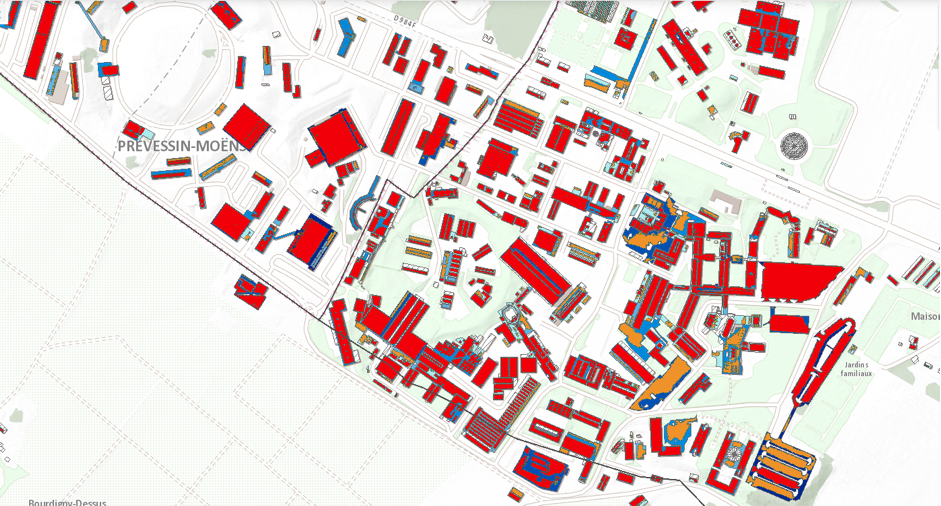
\includegraphics[width=0.8\linewidth]{Energy/ene-cernroof.png}
    \caption[CERN roofs suitable for solar cells]%
        {Map of CERN buildings. Rooftops that are suitable for PV installation in respect to their received solar irradiation are shown in red (very suitable) and yellow (suitable). In addition other areas like \eg parking lots could also be covered by PV-panelled roofs. From Ref.~\cite{SIG}.\label{fig:ene-cernroof}}
    \end{figure}

    Using the cadastre, the cost for electricity from rooftop PV for CERN can be estimated to be fixed around at \EUR{50}/MWh for the next 30 years. This cost is well below current wholesale market spot prices in France (>\EUR{120}/MWh), but also below the average price over summer 2021 (> \EUR{70}/MWh)~\cite{FranceMix}.
\end{casestudy}

%%%%%

\subsubsection{Renewable grid infrastructure}
\label{subsec:grid}
For global power grids to rely more heavily on intermittent sources of renewable energy, such as wind and solar photovoltaic, assessed as having the highest climate mitigation potential to 2030 by the IPCC (see \fref{fig:ene-mitigation}), much of the existing grid infrastructure and controls will need to be updated to smooth out fluctuations in supply and demand~\cite{PowerGridInertia}.  Grid inertia, which acts as a short-term buffer in fossil-fuel grids in periods where electricity demand outstrips supply, is significantly lower for intermittent sources, compromising the stability of the grid. `Smart grid' infrastructure must provide peak-shifting capabilities and fast frequency response to stabilise electricity supply despite the lower intrinsic inertia of the grid.  It will also need to draw upon a novel and expanded energy storage capacity to bridge longer-term gaps between supply and demand~\cite{LDESEnergyStorage} (for further discussion, see below), as well as the capability to regulate bi-directional flow of electricity, well-suited to the distributed generation of intermittents.  Inverter-based resources with low inertia are ideally suited to near-instantaneous response~\cite{PowerGridInertia}.  Electronic control of this response, coupled with developing `grid-forming' technologies, which allow inverters to emulate a traditional grid's stable frequency, as well as automated demand-side response to voluntarily disconnect non-critical loads momentarily, have the potential to transform our existing networks~\cite{PowerGridInertia}.  

Existing solutions have been utilised successfully in several fully renewable island microgrids, and on a larger scale in the Electric Reliability Council of Texas (ERCOT), the smallest of the three power grids in the United States, which achieved 58\% instantaneous wind penetration in 2019 \cite{PowerGridInertia}.  Scaling up these solutions requires further research, although several highly cited studies argue for the feasibility of 100\% renewable-based grids world-wide at low cost, eschewing any fossil fuel or nuclear energy component (for a comprehensive review, see Ref.~\cite{HEARD20171122} and also Ref.~\cite{BROWN2018834}).  

\paragraph{Energy storage}
The feasibility of pure renewable-based grids is crucially dependent on an increased energy storage capacity, to smooth out fluctuations (on timescales ranging from diurnal to seasonal) in the supply of intermittent renewables, and demand~\cite{LDESEnergyStorage}.  While the cost of Li-ion batteries have plummeted 40-fold in the past 35 years~\cite{Ziegler_2020}, their development, driven by needs of the electric vehicle industry, has focused on short-duration portable energy storage.  Projections show that in order to minimise the costs of a net-zero energy system, storage capacity must increase by almost an order of magnitude, from 160 GW (and 9 TWh total capacity) today, to 1.5--2.5 TW (85-140 TWh) globally  by 2040~\cite{LDESEnergyStorage}.  

Most existing and planned storage capacity is in pumped storage hydropower, a mechanical form of storage where water pumped into a reservoir at high elevation turns a turbine as it flows to one at lower elevation~\cite{LDESEnergyStorage}.  As well as being geographically limited, however, these open-air reservoirs suffer the same environmental problems as other hydropower projects (see discussion above), and are similarly subject to the vagaries of the climate. 
A new promising approach to pump storage is the use of undersea bowls that are evacuated to store energy which is restored when they are filled up with water again. An even simpler approach is to build a large ring wall inside of a deep lake, and empty and refill the internal area using pump-turbines. This way, pumped-storage hydroelectricity does not require a separate upper and lower lake, and a single lake is sufficient.
Defunct open pit mines, large natural lakes and even the sea allow for new opportunities to install large-scale storage devices with less environmental impact~\cite{Dueren,pumpstorage}.  

Interesting alternatives include storing energy as compressed air; or as latent heat in, \eg aluminium alloy~\cite{LDESEnergyStorage}.
However, there is need for significant investment in the energy storage sector to bring new ideas, including novel mechanical, thermal, electrochemical and chemical storage methods to commercial viability~\cite{LDESEnergyStorage}.    For more details on capacity and market-readiness of promising long-duration energy storage methods, see Ref.~\cite{LDESEnergyStorage}.


\subsubsection{Energy import and export}
\label{subsec:import}
The uneven geographical distribution of sources of renewable energy leads to the question of whether large-scale import and export of renewable energy could be a cost-effective way of closing the energy gap. For Europe, detailed studies have shown that energy import by cable, as well as by chemical energy carriers, have comparable or lower costs compared to local energy harvesting~\cite{10.1371/journal.pone.0281380}.

Technical options to transport electricity over long distances have improved significantly in the last decades. In South America and China, projects to transport electricity over more than 2,000~km by Ultra High Voltage Direct Current (UHVDC) lines are already operational~\cite{Champion}.

This technological progress opens up an alternative to the traditional import and export of chemical energy: direct import of renewable electricity, e.g., from Northern Africa to Europe~\cite{Dueren,Dueren+2011+263+275}. Indeed, the Xlinks Morocco-UK Power Project~\cite{Xlinks} aims to connect a solar and wind energy facility in Morocco's Guelmim Oued Noun region to the UK energy grid by 3,800 km HVDC sub-sea cables by 2030.

An excellent potential for electricity generation by solar and wind power, large unused tracts of land, and existing energy trade partnerships for fossil fuels make North African countries ideal export partners for procuring electricity from sustainable sources.  \ACR\ has a record of successful collaboration between nations and could thus be an important player in making this happen.  Hence, importing and exporting renewable energy should be considered as part of a catalogue of solutions to cover future global energy needs.  One possible scenario for the transmission of solar energy is detailed in \csref{case:desert}. 

While the import and export of energy is a promising solution on the technical and economic level, constructing wind or solar farms, \eg in the sun belts of Africa, to then export the power to Europe involves geopolitical and social considerations. Resource and person-power extraction from Africa to the benefit of Europe and America has a long, reprehensible colonial history. Therefore, it is of utmost importance to make fair power trade agreements between the continents that ensure strong integration into local communities and include the local population in the planning and implementation of such projects and related infrastructure. In this way, a win-win situation for all stakeholders should be ensured, and well-planned cooperation has the potential to act in a geopolitically stabilizing way in line with the 16th and 17th UN SDGs ("peace, justice and strong institutions" and "partnership for the goals"). 

%%%%%%%%%%%%%%%%%%%%%%%%%%%%%%%%%%%%%%%%%%%%%%%%%% 

\begin{casestudy}[CERN-LINK --- Clean power from the desert\label{case:desert}]{CERN-LINK --- Clean power from the desert}%
The \ACR\ community, CERN in particular, has a long history of effective cooperation across geographical and socio-political boundaries, in the pursuit of science.  
CERN brought scientists from East and West together during the Cold War, and Arabic and Israeli people together for the \acrshort{sesame} project, the first accelerator laboratory powered by solar energy from the desert~\cite{Sesame}. This makes CERN ideally placed to spearhead a project to import solar energy from the deserts of North Africa.  This type of spin-off could help cover CERN's energy needs, while also reinforcing the idea that fundamental research has the potential to solve problems outside its immediate purview in new and innovative ways.\\

%%%%%%%

\begin{figure}
\captionsetup{type=figure}
     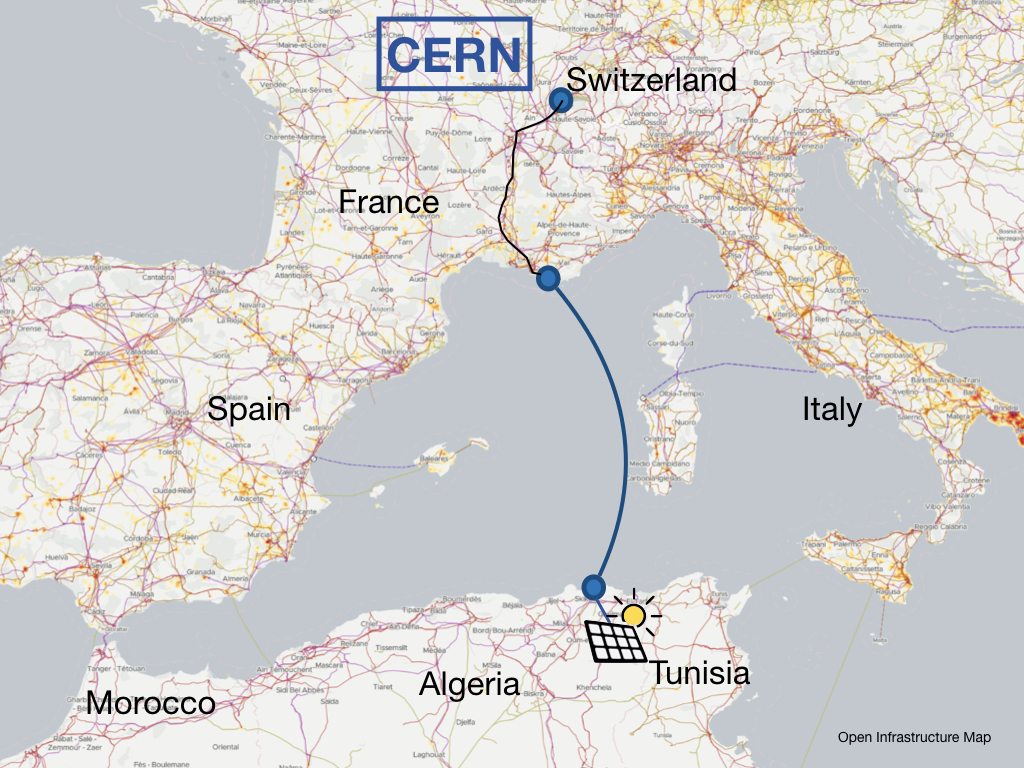
\includegraphics[width=0.7\linewidth]{Energy/ene-cernlink.jpeg}
     \caption[Map for CERN-LINK]{Potential CERN-LINK cable (in blue) connecting North African solar power plants with the European electricity grid. Also shown are existing power lines (purple, red, dashed blue), gas and oil pipelines (green/yellow) and PV plants (yellow/red dots). Base map taken from Ref.~\cite{OpenMap}, reused and annotated under the terms of the \href{https://creativecommons.org/licenses/by/4.0/}{Creative Commons Attribution 4.0 International (CC BY 4.0) license}.}
     \label{fig:ene-cernlink}
\end{figure}

%%%%%%%%%

A scenario for connecting, \eg Morocco, Algeria or Tunisia to Southern France, Spain or Italy by sub-sea cable is plausible from a technological point of view (for a detailed feasibility study, see Ref.~\cite{MoroccoHVDV}), and could be employed for \ACR\ applications (see~\fref{fig:ene-cernlink}). Costs are estimated to be around \EUR{0.06--0.07}/kWh for a year-round power supply of 3.6~GW in the daytime and 2.2~GW at night~\cite{Dueren, Dueren+2011+263+275, Hampp}. This estimate includes infrastructure costs for generating the electricity, buffer storage and transmission line costs. Feasibility and cost estimates agree well with those for previously proposed commercial projects~\cite{Xlinks}.

Electricity imports on this scale would exceed the power needs of CERN, and surplus power could be returned to the European electricity grid to power other research institutions and universities that join the initiative. Southern France is well-suited to the role of import terminal for electricity due to its pre-existing grid infrastructure, as well as its proximity to CERN and other major research institutions. 

It is important to acknowledge that additional environmental considerations are required when planning and implementing a project such as CERN-Link, in terms of minimising the impacts on local ecosystems, as well as the marine environments across which the underwater cables would be installed.  Furthermore, it is of paramount importance that fair power trade agreements be put in place to ensure mutual benefit to all stakeholders, including the local communities hosting the solar infrastructure.

\end{casestudy}


%%%%%%%%%%%%%%%%%%%%%%%%%%%%%%%%%%%%%%%%%%%%%%%%%%

\subsection{Energy Saving and Recuperation}
\label{sec:Ene-Saving}
A first step in reducing energy usage is energy monitoring, which will allow us to assess where improvements are needed. The best energy saving measures will be individual to each location and facility, making it hard to recommend specific actions here, although insulating buildings and ensuring that the heating/ cooling systems are maximally efficient are universally applicable measures. For an example of energy recuperation in the context of basic research, see \bpref{BP:DESY_recycling}.

Most of the energy budget for many high energy experiments is due to the accelerators and detectors. Initiatives to reduce their energy use are many and varied. Relevant references for detectors are collected in \sref{sec:Technology}, see also the discussion on energy saving at \acrshort{lhcb} in \csref{case:LHCb}.  A particularly impressive example of energy-efficient accelerator design is the Cornell-BNL ELR Test Accelerator Facility~\cite{Bartnik:2020pos}, based in Cornell. This accelerator saves energy, both by recovering the energy of the bunched particles to accelerate the next batch, and by using permanent magnets to guide the particle beam.  See \bpref{BP:EnergyRecoveryAccelerator} for more details, and \csref{case:wakefield} for energy savings using plasma wakefield acceleration technology.


\begin{bestpractice}[Recycling energy at DESY\label{BP:DESY_recycling}]{Recycling energy at DESY}%
   For existing experiments, where minimizing energy usage was not a factor in the design process, it is still possible to save energy retroactively through recycling of energy/heat. Deutsches Elektronen-Synchrotron (\acrshort{desy}) is currently using the waste heat that is generated by condensation of the helium that is used to cool the accelerator, to heat their buildings. This saves 7.5 GWh a year, which is approximately a third of the heat energy used on campus~\cite{DESY}. Together with the University for Applied Sciences in Hamburg, they are also investigating the potential for recycling waste heat from other sources, \eg the many magnets used in the accelerator. First results suggest it should be sufficient to heat all buildings on campus in this way~\cite{DESYsustainableReport2022}.
\end{bestpractice}

\end{document}
